\section{Introducci\'on}
En este problema, se nos pide que ideemos un algoritmo que dados $n$ productos quimicos que deben transportarse en camiones de un lugar a otro, tales que si un elemento $i$ va en el mismo cambion que otro elemento $j$, esto conlleva una "peligrosidad" asociada $h_i_j$. El objetivo aqu\'i es utilizar la menor cantidad de cami\'ones posibles, pero que cada cami\'on tenga una peligrosidad menor a una cota $m$.
\\
La entrada del problema consiste en:
\\
\begin{itemize}
\item Un entero \textbf{n} $\rightarrow$ Representar\'an el n\'umero de productos quimicos a transportar.
\item Un entero \textbf{m} $\rightarrow$ Representar\'a la cota de peligrosidad que ningun cami\'on puede superar.
\item \textbf{n-1} filas donde, para cada fila $i$ consta de $n-i$ enteros:
\begin{itemize}
\item $h_i_{i+1}, h_i_{i+2}$ ... $h_i_{n}$ $\rightarrow$ Representar\'an la peligrosidad asociada del elemento $i$ con los elementos $i+1$, $i+2$ ... $n$.
\end{itemize}
\end{itemize}
\\
La salida, por su parte, constar\'a de una fila con:
\\
\begin{itemize}
\item Un entero \textbf{C} $\rightarrow$ Representar\'a la cantidad indispensable de cami\'ones que es necesaria para transportar los productos bajo las condiciones del problema.
\item $n$ enteros $\rightarrow$ Representar\'an en que cami\'on viaja cada producto.
\end{itemize}

\subsection{Ejemplo de entrada valida}
Hagamos un pequeño ejemplo para que pueda ilustrarse bien el problema.
\\
Supongamos que tenemos $3$ productos quimicos, el producto $1$ es muy inestable, por lo que si es transportado con el producto $2$ la peligrosidad asciende a $40$, y si se transporta con el producto $3$ la peligrosidad es de $35$. El producto $2$ en cambio es de naturaleza mas estable, por lo que si es transportado con el producto $3$ solo produce una peligrosidad de $3$.
\\
Por otro lado queremos que la peligrosidad por cami\'on no supere el valor de $39$.
\\
Entonces la entrada para este problema ser\'a:
\\
\\
$\textbf{3 39}$
\\
$\textbf{40 35}$
\\
$\textbf{3}$
\\
\\
Para una entrada de estas dimenciones es posible buscar la mejor solucio\'on a mano.
\\
Las posibles combinaciones son que los tres productos viajen juntos, que los tres viajen separados, que $1$ y $2$ viajen juntos, que $1$ y $3$ viajen juntos y que $2$ y $3$ viajen juntos y el producto sobrante viaje en otro cami\'on.
\\
La primera d\'a una peligrosidad de $40+35+3$ por lo que es inviable, la segunda es valida, pero se necesitan $3$ camiones. Que $1$ y $2$ viajen juntos, tampoco es valida (peligrosidad muy alta), y finalmente las ultimas dos son validas (peligrosidad $35$ y $3$, respectivamente) y solo son necesarios dos camiones.
\\
Luego las dos salidas que podr\'a devolver el algoritmo son:
\begin{itemize}
\item $2$ $1$ $2$ $1$
\end{itemize}
o
\begin{itemize}
\item $2$ $1$ $2$ $2$
\end{itemize}
\\
\section{Idea General de Resoluci\'on}
Luego la idea del algoritmo es simple, probar todas las combinaciones posibles de camiones y de entre todas determinar cual es la que cumple con la cota de peligrosidad pedida y usa la menor cantidad de camiones posible. Ademas, se ir\'a podando algunas ramas de una manera mas o menos inteligente para intentar lograr una mejor performance.
\\
Antes de presentar el pseudocodigo vale aclarar un punto importante y es que este algoritmo encontra\'a siempre una soluci\'on. Esto se debe a que siempre es posible poner todos los productos quimicos en camiones separados, lo que nos d\'a  una peligrosidad $0$. Luego es posible usar esta como una cota contra la cual parar de chequear, si tenemos $n$ productos quimicos, es simple ver que a lo sumo usar\'emos $n$ camiones. Denominaremos a esta como la "peor soluci\'on" ya que es claro que es una soluci\'on valida, pero que usa la maxima cantidad de camiones.
\\
En cuanto a las podas, utilizamos dos, una que en cada paso del backtrack chequea si la soluci\'on final que encontramos hasta el momento usa una cantidad menor de camiones que la solucion parcial que se esta construyendo. Es claro que de ser as\'i, estamos la solucion parcial nunca podr\'a ser mejor, por lo tanto se poda.
\\
La segunda chequea que la soluci\'on parcial que estamos construyendo no exceda el limite de peligrosidad pedido por el ejercicio. En caso de que esto suceda, tambien se poda.
\\
Finalmente el pseudocodigo para resolver este problema queda as\'i:

\begin{algorithm}
\begin{algorithmic}[1]\parskip=1mm
\caption{void FuncionPrincipal()}

  \STATE{Generar una matriz con las peligrosidades entre los distintos productos}
  
  \STATE{Se inicializa la solucion final, como la peor de las soluciones}
  
  \STATE{Backtrack(tabla_de_peligrosidad, solucion_parcial, solucion_final)}
  
  \STATE{Mostar la soluci\'on final}
 
 \end{algorithmic}
\end{algorithm}

\begin{algorithm}
\begin{algorithmic}[1]\parskip=1mm
\caption{Bool Backtrack(tabla_de_peligrosidad, solucion_parcial, solucion_final)}
	
	\STATE{Llamo a la funcion check(tabla_de_peligrosidad, solucion_parcial, solucion_final)}
	
	\STATE{\quad Si check devuelve $2$, la solucion parcial es mejor que la final}
	\STATE{\quad \quad Pongo la solucion parcial como final} 
	\STATE{\quad \quad Corto la recursi\'on y busco por otra rama}

	\STATE{\quad Si check devuelve $3$, la solucion anterior usa menos camiones}
	\STATE{\quad \quad esta rama no me sirve, podo}

	\STATE{\quad Si check devuelve $0$, la cota de peligrosidad fu\'e sobrepasada}
	\STATE{\quad \quad esta rama no me sirve, podo}

	\STATE{\quad Si check devuelve $1$, la solucion es valida, pero no est\'a completa}
	\STATE{\quad \quad contin\'uo agregando camiones}

	\STATE{Para cada valor $i$ de $1$ hasta $n$ prueba meter el siguiente producto de la lista en el camion $i$ y se llama a la funcion Backtrack()}
\end{algorithmic}
\end{algorithm}

\begin{algorithm}
\begin{algorithmic}[1]\parskip=1mm
\caption{int check(tabla_de_peligrosidad, solucion_parcial, solucion_final)}


\STATE{Checkeo si la solucion final usa menos camiones ~~~~~~~~~~~~ $O(n)$}
\STATE{\quad Si es verdad}
\STATE{\quad \quad Devuelvo $3$}


\STATE{Checkeo si la cota de peligrosidad fue sobrepasada ~~~~~~~~~~~~ $O(n^2)$}
\STATE{\quad Si es verdad}
\STATE{\quad \quad Devuelvo $0$}


\STATE{Checkeo si la cada producto tiene un camion asignado ~~~~~~~~~~~~ $O(1)$}
\STATE{\quad Si es verdad}
\STATE{\quad \quad Devuelvo $2$}

\STATE{Devuelvo $1$}

\end{algorithmic}
\end{algorithm}


\newpage
\section{Complejidad}
Por cada producto quimico, el algoritmo de backtrack intenta ponerlo en cualquiera de los $n$ posibles camiones, y realiza $O(n^2)$ chequeos intentando podar.
\\
Entonces la formula quedar\'a:
\\
$$T(i) = T(i-1)n + n^2$$
\\
$$T(1) = n + n^2$$
\\
Luego para el peor de los casos el algoritmo tendr\'a una complejidad de $O(n^n)$.
\\
\section{Testing}
\subsection{Caso Random}
Para testear la performance de nuestro algoritmo se cre\'o un generador de entradas que fabricar\'a instancias random del problema. Luego se comparar\'a el tiempo que tarda nuestro algoritmo contra uno que encuentre la soluci\'on utilizando fuerza bruta y tambien contra otro backtraking, pero con las podas invertidas, osea primero chequea si la cantidad de camiones de la solucion parcial es menor a la cantidad de camiones de la mejor soluci\'on hasta el momento y luego chequea que la cota de complejidad sea la correcta, para ver si esto var\'ia de alguna manera la complejidad.
\\
El testeo consistio en generar 40 instancias del problema para cada $n$ diferente (con un $m$ fijo), luego se tom\'o la media y graficaron los resultados:
\\
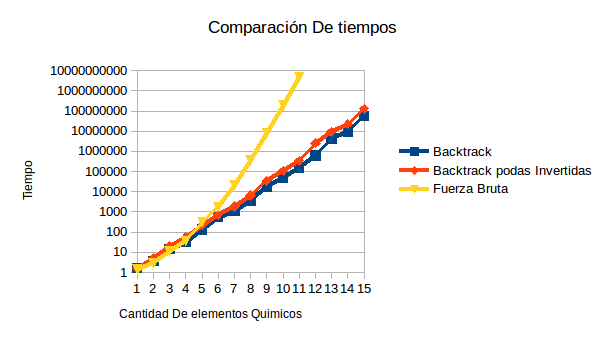
\includegraphics[width=18cm]{./Ej3/graph1.png}
\\
En este grafico puede verse que nuestro algoritmo es notablemente superior a uno algoritmo de fuerza bruta y levemente mejor al backtraquing con las podas invertidas. Para los casos de $14$ y $15$ elementos el backtraking pudo arrojar una respuesta en un tiempo admisible, mientras que el de fuerza bruta ya tardaba tiempos completamente fuera de escala.
\\
Se relai\'o lo mismo variando la cota de peligrosidad $m$ para ver como se ve\'ian afectados los diversos algoritmos ($n$ = $9$):
\\
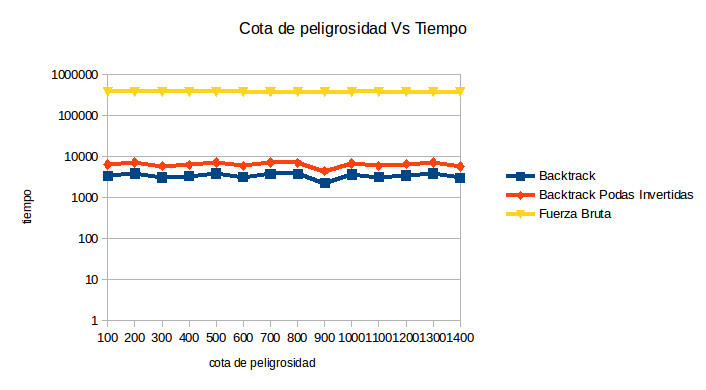
\includegraphics[width=18cm]{./Ej3/graph2.png}
\\
La clara concluci\'on es que ningun algoritmo se ve afectado por la cota de peligrosidad.

\subsection{Peor caso}
Otro test que podemos intentar realizar es ver si nuetro algormitmo presenta alguna mejora al de fuerza bruta en el peor de los casos, esto es, en el caso de que cada producto tenga que viajar forzosamente en un camion diferente.
\\
Para testear esto tomamos nuevamente $40$ entradas y las corremos en los tres algoritmos.



\newpage
\section{Resultados}